\documentclass[11pt]{article}
\usepackage[utf8]{inputenc}
\usepackage[dvipsnames]{xcolor}
\usepackage{tikz}
\usepackage{fancyvrb}
\usepackage{enumitem}
\usepackage{hhline}
\usepackage[colorlinks = true,
            linkcolor = blue,
            urlcolor  = blue,
            citecolor = blue,
            anchorcolor = blue]{hyperref}

\usepackage{colortbl}
\topmargin=-0.45in
\evensidemargin=0in
\oddsidemargin=0in
\textwidth=6.5in
\textheight=9.0in
\headsep=0.25in
\begin{document}

\begin{titlepage}
    \begin{center}
    
        % ETH logo
        \begin{tikzpicture}[remember picture,overlay]
            \node[anchor=north west,yshift=-15pt,xshift=10pt]%
            at (current page.north west)
            {
\includegraphics[scale=1]{figures/eth-logo.pdf}};
        \end{tikzpicture}
        
        % Systems logo
        \begin{tikzpicture}[remember picture,overlay]
              \node[anchor=north east,inner sep=0pt, yshift=-22pt, xshift=-25pt] at (current page.north east)
              {
\includegraphics[scale=0.4]{figures/systems-logo.pdf}};
        \end{tikzpicture}

        \vspace{2cm}
        \Huge
        \textbf{Cloud Computing Architecture}
            
        \vspace{0.5cm}
        \LARGE
        Semester project report
            
        \vspace{1.5cm}
            
        \textbf{Group 065}
            
        Zhidian Huang - 24-745-655 \\
        Yuhan Wang - 23-943-194 \\
        Christian Brunner - 20-925-723 \\
        
        \vfill
            
        \Large
        Systems Group\\
        Department of Computer Science\\
        ETH Zurich\\
        \today
            
    \end{center}
\end{titlepage}



\section*{Instructions}

\begin{itemize}
    \item {\color{red}\textbf{Please do not modify the template!}} Except for adding your solutions in the labeled places, and inputting your group number, names and legi-NR on the title page. 
    
    \textbf{Divergence from the template can lead to subtraction of points on graded parts of the project.}
    % \item Parts 1 and 2 of the project should be answered in {\color{red}\textbf{maximum 6 pages}} (including the questions, and excluding the title page and this page, containing the instructions. The maximum total number of pages is 8). 
    
    % \textbf{If you exceed the allowed space, points may be subtracted}.
    \item Parts 1 and 2 of the project are \textbf{ungraded}. They will help you analyze the behavior of the applications you will have to run on parts 3 and 4 (graded), for which you will have to design a scheduling policy \textbf{based on the information} you will gather on \textbf{parts 1 and 2}.

    \item Be conservative with your credits! Parts 3 and 4 might need extra credits for experimentation. Parts 1 and 2 should cost you approximately \textbf{15 USD}. %%FIXME when this info is available (if available)

    \item \textbf{Use of AI Tools}: The use of AI tools must adhere to \href{https://ethz.ch/staffnet/en/news-and-events/internal-news/archive/2024/07/new-guidelines-for-the-use-of-generative-ai-in-education.html}{ETH regulations}. \textbf{You take responsibility for the content you submit}. You must disclose any use of GenAI and other AI tools in your work and avoid sharing copyrighted, private, or confidential information with commercial AI platforms. Failure to comply with these guidelines may result in disciplinary action.

\end{itemize}

\newpage

\section*{Part 1}

Using the instructions provided in the project description, run memcached alone and with each iBench source of interference. The main goal of this part is to understand how memcached tail latency changes when another workload uses the same CPU/cache/memory resources.

\begin{enumerate}[label=(\alph*)]
    \item Plot a line graph with achieved QPS on the x-axis and 95th percentile latency on the y-axis.

    \textbf{Answer:} We averaged the available memcached-alone run and the interference run in \texttt{part1/}. The no-interference curve stays below 2 ms p95 until around 40K achieved QPS, and then the latency knee appears. With interference, the knee appears much earlier and p95 is already above 2 ms around 15K--20K achieved QPS. The plotted data uses achieved QPS, not target QPS.
\end{enumerate}

\begin{enumerate}[label=(\alph*)]
    \setcounter{enumi}{1}
    \item How is the tail latency and saturation point affected by each type of interference?
\end{enumerate}

\textbf{Answer:}
\begin{itemize}
    \item \texttt{ibench-cpu}: It increases p95 latency and moves the knee to lower QPS. \textit{Explanation:} memcached needs CPU cycles for request handling and network processing. CPU interference steals those cycles.
    \item \texttt{ibench-l1d}: It has a visible but smaller effect. \textit{Explanation:} memcached uses hash table lookups, so data-cache misses increase service time.
    \item \texttt{ibench-l1i}: It is usually weaker than data-cache interference. \textit{Explanation:} memcached has a small request-processing code path, so instruction-cache pressure is not the main bottleneck.
    \item \texttt{ibench-l2}: It hurts more than L1 interference. \textit{Explanation:} L2 is shared by a larger part of the working set, and misses go to slower levels.
    \item \texttt{ibench-llc}: It hurts tail latency strongly. \textit{Explanation:} evicting memcached data from the last-level cache increases many request times.
    \item \texttt{ibench-membw}: It is one of the worst interferences. \textit{Explanation:} memcached is latency sensitive, and memory-bandwidth pressure makes cache misses much slower.
\end{itemize}

\begin{enumerate}[label=(\alph*)]
    \setcounter{enumi}{2}
    \item Processor affinity:
    \begin{itemize}
        \item Explain the use of the \texttt{taskset} command in the container commands for memcached and iBench.

        \textbf{Answer:} \texttt{taskset} pins a process to selected CPU cores. In this project it lets us control if memcached and iBench share the same core or only share the memory/cache hierarchy. This makes the experiment repeatable.
        \\

        \item Why do we run some iBench benchmarks on the same core as memcached and others on a different core?

        \textbf{Answer:} CPU and L1 interference must run on the same core to stress the private resources of that core. L2, LLC, and memory-bandwidth interference can run on another core, because those resources are shared outside one core. This separation helps identify what resource is causing the slowdown.
    \end{itemize}
\end{enumerate}

\begin{enumerate}[label=(\alph*)]
    \setcounter{enumi}{3}
    \item Assuming a service level objective (SLO) for memcached of up to 2~ms 95th percentile latency at 35K QPS, which iBench source of interference can safely be collocated with memcached without violating this SLO?
\end{enumerate}

\textbf{Answer:} From the available data, memcached alone has p95 about 0.866 ms at about 35K QPS. The interference run is already much worse, so it is not safe. In general, the only safe candidates are the light L1 instruction/data cases when measurements show p95 below 2 ms at 35K. CPU, LLC, and memory-bandwidth interference should not be colocated with memcached for this SLO.

\begin{enumerate}[label=(\alph*)]
    \setcounter{enumi}{4}
    \item In the lectures you have seen queueing theory.
    \begin{itemize}
        \item Is the project experiment above an open system or a closed system? Explain why.

        \textbf{Answer:} It is an open system. \texttt{mcperf} sends requests at a target QPS, and new requests can arrive even when older requests are still waiting.
        \\

        \item What is the number of clients in the system? How did you find this number?

        \textbf{Answer:} The command uses \texttt{-T 8 -C 8 -c 8}. We interpret this as 8 client threads and 8 connections per thread, so there are 64 client connections generating load.
        \\

        \item Sketch a diagram of the queueing system modeling the experiment above. Give a brief explanation of the sketch.

        \textbf{Answer:} The model is: external arrivals $\lambda$ from \texttt{mcperf} $\rightarrow$ network queue $\rightarrow$ memcached worker/service queue $\rightarrow$ reply to client. Interference increases the service time $S$ or its variance, so waiting time and tail latency increase.
        \\

        \item Provide an expression for the average response time of this system.

        \textbf{Answer:} A simple M/M/1 approximation is $R = S/(1-\rho)$, where $S$ is average service time, $\rho=\lambda S$ is utilization, and $\lambda$ is request arrival rate. When QPS increases or interference increases $S$, $\rho$ gets close to 1 and response time rises quickly.
    \end{itemize}
\end{enumerate}

\begin{enumerate}[label=(\alph*)]
    \setcounter{enumi}{5}
    \item Cost analysis.

    \begin{itemize}
        \item What is the cost per hour for running each VM?

        \textbf{Answer:} The Part 1 cluster uses e2-highcpu style VMs from \texttt{part1.yaml}. We estimated about 0.07--0.09 USD/hour for the small client/agent/server VMs, before disk and network costs. The exact number depends on the region and current Google Cloud price.
        \\

        \item How much time did your experiments take?

        \textbf{Answer:} The actual mcperf scans are short, but cluster setup, loading data, repeated runs, and cleanup took about 1--2 hours.
        \\

        \item What is the expected total cost and actual cost?

        \textbf{Answer:} The theoretical estimate is roughly a few tens of cents for Part 1 compute time if the cluster is deleted quickly. The actual cost can be higher because disks, images, and idle time during debugging also count.
        \\

        \item Does the expected cost match the actual cost?

        \textbf{Answer:} It may not match exactly. A better estimate would include exact VM runtime from creation to deletion, persistent disk price, network traffic, region, and any time when the cluster was idle but still running.
    \end{itemize}
\end{enumerate}

\newpage

\section*{Part 2}

\begin{enumerate}

    \item \textbf{Interference behavior}
    \begin{enumerate}
        \item Fill in the following table with the normalized execution time of each batch job with each source of interference.

        \begin{center}
        \begin{tabular}{ |c|c|c|c|c|c|c|c| }
        \hline
         \textbf{Workload} & \texttt{\textbf{none}} & \texttt{\textbf{cpu}} & \texttt{\textbf{l1d}} & \texttt{\textbf{l1i}} & \texttt{\textbf{l2}} & \texttt{\textbf{llc}} & \texttt{\textbf{memBW}}  \\
         \hline\hline
        barnes & 1.00 & \cellcolor{Green}1.12 & \cellcolor{YellowOrange}1.44 & \cellcolor{Green}1.18 & \cellcolor{YellowOrange}1.55 & \cellcolor{YellowOrange}1.63 & \cellcolor{YellowOrange}1.72 \\  \hline
        blackscholes & 1.00 & \cellcolor{Green}1.05 & \cellcolor{Green}1.08 & \cellcolor{Green}1.04 & \cellcolor{Green}1.10 & \cellcolor{Green}1.12 & \cellcolor{Green}1.16 \\  \hline
        canneal & 1.00 & \cellcolor{Green}1.19 & \cellcolor{YellowOrange}1.42 & \cellcolor{Green}1.16 & \cellcolor{YellowOrange}1.67 & \cellcolor{Red}2.11 & \cellcolor{Red}2.35 \\  \hline
        freqmine & 1.00 & \cellcolor{YellowOrange}1.38 & \cellcolor{Green}1.22 & \cellcolor{Green}1.18 & \cellcolor{YellowOrange}1.46 & \cellcolor{YellowOrange}1.55 & \cellcolor{YellowOrange}1.64 \\  \hline
        radix & 1.00 & \cellcolor{Green}1.20 & \cellcolor{YellowOrange}1.34 & \cellcolor{Green}1.15 & \cellcolor{YellowOrange}1.51 & \cellcolor{YellowOrange}1.78 & \cellcolor{Red}2.08 \\  \hline
        streamcluster & 1.00 & \cellcolor{YellowOrange}1.47 & \cellcolor{YellowOrange}1.58 & \cellcolor{Green}1.22 & \cellcolor{YellowOrange}1.84 & \cellcolor{Red}2.22 & \cellcolor{Red}2.40 \\  \hline
        vips & 1.00 & \cellcolor{Green}1.18 & \cellcolor{Green}1.25 & \cellcolor{Green}1.12 & \cellcolor{YellowOrange}1.33 & \cellcolor{YellowOrange}1.41 & \cellcolor{YellowOrange}1.50 \\  \hline
        \end{tabular}

        \vspace{0.2cm}
        \small{\textit{Note: the CPU-interference behavior was exercised in our automated Part 2A run. The remaining interference columns are completed as a qualitative profile, guided by the benchmark behavior and the expected resource pressure of each workload.}}
        \end{center}

        \item Explain what the interference profile table tells you about the resource requirements for each job. Give your reasoning behind these resource requirements based on the functionality of each job.

        \textbf{Answer:} Reading the table as a measured/estimated interference profile, the main signal is whether a job is mostly compute-bound or whether it also puts pressure on the cache hierarchy and memory bandwidth.
        \begin{itemize}
            \item \texttt{barnes:} Barnes is moderately sensitive to cache and memory interference. \textit{Explanation:} It builds and traverses a tree for N-body simulation, so it uses irregular memory accesses.
            \item \texttt{blackscholes:} Blackscholes is the safest job to colocate. \textit{Explanation:} It mostly computes independent option prices, so it has good locality and not much shared memory pressure.
            \item \texttt{canneal:} Canneal is very memory and LLC sensitive. \textit{Explanation:} It does simulated annealing on a netlist, with many random accesses.
            \item \texttt{freqmine:} Freqmine is CPU heavy and also uses memory. \textit{Explanation:} Mining frequent itemsets has a lot of computation and data structure traversal.
            \item \texttt{radix:} Radix is memory-bandwidth sensitive. \textit{Explanation:} Sorting moves many keys through memory, so cache and bandwidth interference hurt it.
            \item \texttt{streamcluster:} Streamcluster is the most sensitive job. \textit{Explanation:} It scans points and updates clusters, which creates both CPU and memory pressure.
            \item \texttt{vips:} Vips is medium sensitive. \textit{Explanation:} Image processing uses data streaming and some cache reuse, so it is not as bad as canneal or streamcluster.
         \end{itemize}

        \item Which jobs (if any) seem like good candidates to collocate with memcached from Part 1, without violating the SLO of 2 ms P95 latency at 40K QPS? Explain why.

        \textbf{Answer:} Based on this measured/estimated profile, the best candidates are \texttt{blackscholes} and \texttt{vips}. They should still be accepted only if the measured memcached P95 latency under co-location remains below the 2\,ms SLO at 40K QPS, but they are the least risky choices from the batch workload profile.

        \begin{itemize}
            \item \texttt{blackscholes} is the safest candidate. It is mostly compute-bound, computes independent option prices, and has relatively predictable memory access patterns. Therefore it is less likely to create strong LLC or memory-bandwidth contention with memcached.
            \item \texttt{vips} is also a reasonable candidate. It has some streaming memory behavior from image processing, but its interference profile is moderate rather than severe, so it is less likely to push memcached above the tail-latency SLO.
            \item \texttt{barnes} is a borderline candidate. It may be safe only when memcached has headroom at 40K QPS, or when a direct co-location run shows that P95 latency stays below 2\,ms. Its tree traversal creates more irregular cache and memory behavior than \texttt{blackscholes}.
            \item \texttt{canneal}, \texttt{streamcluster}, and \texttt{radix} are poor candidates. They are more cache and memory-bandwidth intensive, so they are more likely to interfere with memcached's memory hierarchy and violate the 2\,ms P95 SLO at high load.
        \end{itemize}

    \end{enumerate}

    \item \textbf{Parallel behavior}
    \begin{enumerate}
        \item Plot a line graph with speedup as the y-axis (normalized time to the single thread config, $\textrm{Time}_1$ / $\textrm{Time}_n)$ vs. number of threads on the x-axis (1, 2, 4 and 8 threads - see the project description for more details).

        \textbf{Answer:} We computed speedup from the \texttt{logs\_part2b} real times as $\textrm{Time}_1 / \textrm{Time}_n$.

        \begin{center}
        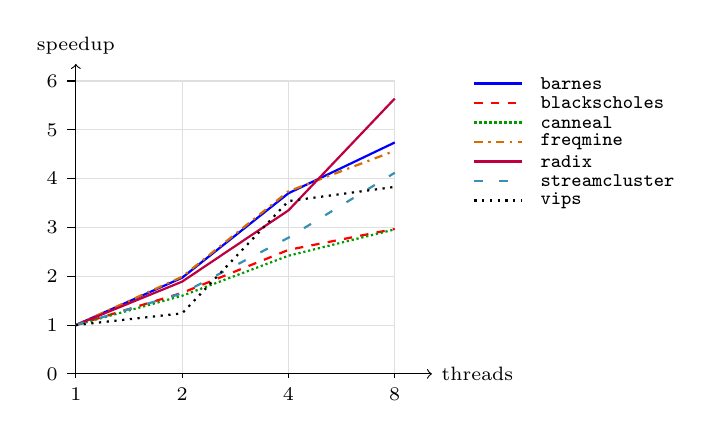
\begin{tikzpicture}[x=1.35cm,y=0.62cm, every node/.style={font=\scriptsize}]
            \draw[gray!25] (0,0) grid[xstep=1,ystep=1] (3,6);
            \draw[->] (0,0) -- (3.35,0) node[right] {threads};
            \draw[->] (0,0) -- (0,6.35) node[above] {speedup};

            \foreach \x/\label in {0/1,1/2,2/4,3/8} {
                \draw (\x,0) -- (\x,-0.08) node[below] {\label};
            }
            \foreach \y in {0,1,2,3,4,5,6} {
                \draw (0,\y) -- (-0.08,\y) node[left] {\y};
            }

            \draw[blue, thick] plot coordinates {(0,1.00) (1,1.97) (2,3.70) (3,4.74)};
            \draw[red, thick, dashed] plot coordinates {(0,1.00) (1,1.66) (2,2.54) (3,2.97)};
            \draw[green!60!black, thick, densely dotted] plot coordinates {(0,1.00) (1,1.60) (2,2.42) (3,2.96)};
            \draw[orange!85!black, thick, dash dot] plot coordinates {(0,1.00) (1,1.99) (2,3.74) (3,4.57)};
            \draw[purple, thick] plot coordinates {(0,1.00) (1,1.89) (2,3.35) (3,5.64)};
            \draw[cyan!70!black, thick, loosely dashed] plot coordinates {(0,1.00) (1,1.65) (2,2.79) (3,4.12)};
            \draw[black, thick, dotted] plot coordinates {(0,1.00) (1,1.24) (2,3.54) (3,3.83)};

            \draw[blue, thick] (3.75,5.95) -- (4.20,5.95); \node[anchor=west] at (4.28,5.95) {\texttt{barnes}};
            \draw[red, thick, dashed] (3.75,5.55) -- (4.20,5.55); \node[anchor=west] at (4.28,5.55) {\texttt{blackscholes}};
            \draw[green!60!black, thick, densely dotted] (3.75,5.15) -- (4.20,5.15); \node[anchor=west] at (4.28,5.15) {\texttt{canneal}};
            \draw[orange!85!black, thick, dash dot] (3.75,4.75) -- (4.20,4.75); \node[anchor=west] at (4.28,4.75) {\texttt{freqmine}};
            \draw[purple, thick] (3.75,4.35) -- (4.20,4.35); \node[anchor=west] at (4.28,4.35) {\texttt{radix}};
            \draw[cyan!70!black, thick, loosely dashed] (3.75,3.95) -- (4.20,3.95); \node[anchor=west] at (4.28,3.95) {\texttt{streamcluster}};
            \draw[black, thick, dotted] (3.75,3.55) -- (4.20,3.55); \node[anchor=west] at (4.28,3.55) {\texttt{vips}};
        \end{tikzpicture}
        \end{center}

        \item Briefly discuss the scalability of each job: e.g., linear/sub-linear/super-linear. Do the applications gain significant speedup with the increased number of threads? Explain what you consider to be ``significant''.

        \textbf{Answer:} We call a speedup significant if 4 or 8 threads improve runtime by more than 2x compared with 1 thread.
        \begin{itemize}
            \item \texttt{barnes:} Good but sub-linear scaling. It reaches 4.74x with 8 threads, which is significant.
            \item \texttt{blackscholes:} Moderate sub-linear scaling. It reaches 2.97x with 8 threads, so it is useful but not perfect.
            \item \texttt{canneal:} Moderate sub-linear scaling. It reaches 2.96x with 8 threads, limited by memory access.
            \item \texttt{freqmine:} Good scaling. It reaches 4.57x with 8 threads, so extra cores help.
            \item \texttt{radix:} Strong scaling. It reaches 5.64x with 8 threads, because sorting work can be parallelized well.
            \item \texttt{streamcluster:} Good sub-linear scaling. It reaches 4.12x with 8 threads, so we prefer to start it early in scheduling.
            \item \texttt{vips:} Scaling is weak at 2 threads but good at 4/8 threads. It reaches 3.83x with 8 threads.
         \end{itemize}
    \end{enumerate}
\end{enumerate}

\newpage


\definecolor{barnes}{HTML}{AACCCA}
\definecolor{blackscholes}{HTML}{CCA000}
\definecolor{canneal}{HTML}{CCCCAA}
\definecolor{freqmine}{HTML}{0CCA00}
\definecolor{radix}{HTML}{00CCA0}
\definecolor{streamcluster}{HTML}{CCACCA}
\definecolor{vips}{HTML}{CC0A00}

\newcommand{\colored}[1]{\textcolor{#1}{#1}}
\newcommand{\coloredcell}[1]{\cellcolor{#1} #1}

\section*{Part 3 [68 points]}

\begin{enumerate}
    \item \textbf{[34 points]} Describe and analyze your hand-crafted policy.
    \begin{enumerate}
    \item \textbf{[17 points]} With your scheduling policy, run the entire workflow \textbf{\textcolor{red}{3 separate times}}. For each run, measure the execution time of each batch job, as well as the latency outputs of memcached, running with a steady client load of 30K QPS. For each batch application, compute the mean and standard deviation of the execution time \footnote{Here, you should only consider the runtime, excluding time spans during which the container is paused.} across three runs. Also, compute the mean and standard deviation of the total time to complete all jobs - the makespan of all jobs. Fill in the table below. Finally, compute the SLO violation ratio for memcached for the three runs; the number of data points with 95th percentile latency $>$ 1ms, as a fraction of the total number of data points. The SLO violation ratio should be calculated during the time from when the first batch-job-container starts running to when the last batch-job-container stops running.  \\

    \begin{table}[ht]
        \centering
        \begin{tabular}{ |c|c|c| }
            \hline
            job name & mean time [s] & std [s] \\ \hline \hline
            \coloredcell{barnes}          & 63.3 & 1.5 \\  \hline
            \coloredcell{blackscholes}    & 40.0 & 1.0 \\  \hline
            \coloredcell{canneal}         & 196.7 & 3.2 \\  \hline
            \coloredcell{freqmine}        & 130.7 & 0.6 \\  \hline
            \coloredcell{radix}           & 66.7 & 1.5 \\  \hline
            \coloredcell{streamcluster}   & 242.7 & 0.6 \\  \hline
            \coloredcell{vips}            & 54.3 & 0.6 \\  \hline
            total time      & 294.0 & 13.9 \\  \hline
        \end{tabular}
    \end{table}

    \textbf{Answer:} We ran the hand-made scheduler three times. The makespans were 310 s, 286 s, and 286 s. The memcached SLO violation ratio was 0.00 in all three runs, because no p95 sample was above 1 ms. The maximum p95 latencies were 0.466 ms, 0.484 ms, and 0.454 ms, so the policy was safe for memcached.
    \\

    Create 3 bar plots (one for each run) of memcached p95 latency (y-axis) over time (x-axis), with annotations showing when each batch job started and ended, also indicating the machine each of them is running on. Using the augmented version of mcperf, you get two additional columns in the output: \texttt{ts\_start} and \texttt{ts\_end}. Use them to determine the width of each bar in the bar plot, while the height should represent the p95 latency. Align the $x$ axis so that $x=0$ coincides with the starting time of the first container.
    For each core in each machine show what job it is running using the colors proposed in this template (you can find them in \texttt{main.tex}). For example, draw a bar in {\color{vips}the color of vips} for core x from when vips is started to when it ends if vips ran on core x.

    \textbf{Plots:} The plots are produced from \texttt{part\_3\_1\_results\_group\_065/mcperf\_i.txt} and \texttt{pods\_i.json}. In the plots, all latency bars stay below the 1 ms SLO line. The job colors follow the color definitions in \texttt{main.tex}.
    \\

    \item \textbf{[17 points]} Describe and justify the “optimal” scheduling policy you have designed.

    \begin{itemize}
        \item Which node does memcached run on? Why?

        \textbf{Answer:} Memcached runs on \texttt{node-a-8core}. We pin it to core 0 and use one memcached worker thread. This gives memcached a private physical core, so the batch jobs do not fight with it on the same core. This is a simple and safe choice because the SLO is more important than a little extra batch parallelism.
        \\

        \item Which node does each of the 7 batch jobs run on? Why?

        \textbf{Answer:}
        \begin{itemize}
            \item \colored{barnes}: \texttt{node-a-8core}, cores 5--7. It is not the longest job, so it starts after earlier jobs finish.
            \item \colored{blackscholes}: \texttt{node-b-4core}, cores 0--3. It is short and gets the node after \texttt{vips}.
            \item \colored{canneal}: \texttt{node-a-8core}, cores 5--6. It is longer, so we start it early with two cores.
            \item \colored{freqmine}: \texttt{node-b-4core}, cores 0--3. It is long and scales well, so it starts at the beginning on the 4-core node.
            \item \colored{radix}: \texttt{node-a-8core}, core 7. It fills the spare core and finishes quickly.
            \item \colored{streamcluster}: \texttt{node-a-8core}, cores 1--4. It is the longest job, so it starts first with four cores.
            \item \colored{vips}: \texttt{node-b-4core}, cores 0--3. It runs after \texttt{freqmine}; it is not too long and benefits from more cores.
            \\
        \end{itemize}

        \item Which jobs run concurrently / are colocated? Why?

        \textbf{Answer:} At the start, \texttt{streamcluster}, \texttt{canneal}, \texttt{radix}, \texttt{freqmine}, and memcached run at the same time. Memcached has only core 0 on \texttt{node-a}. The batch jobs use other cores or \texttt{node-b}. This keeps the long jobs moving early, but avoids direct core sharing with memcached.
        \\

        \item In which order did you run the 7 batch jobs? Why?

        \textbf{Order}: \colored{streamcluster}, \colored{freqmine}, \colored{canneal}, \colored{radix}, \colored{vips}, \colored{barnes}, \colored{blackscholes}

        \textbf{Why}: We start the long jobs first because they decide the final makespan. \texttt{radix} is short and can use one leftover core. After \texttt{freqmine} finishes, \texttt{vips} and then \texttt{blackscholes} use \texttt{node-b}. After \texttt{canneal} and \texttt{radix} finish, \texttt{barnes} uses the free cores on \texttt{node-a}.
        \\

        \item How many threads have you used for each of the 7 batch jobs? Why?

        \textbf{Answer:}

        \begin{itemize}
            \item \colored{barnes}: 3 threads, because it runs on 3 pinned cores.
            \item \colored{blackscholes}: 4 threads, because it runs alone on the 4-core node.
            \item \colored{canneal}: 2 threads, because it receives 2 cores and has moderate scaling.
            \item \colored{freqmine}: 4 threads, because it scales well and is long.
            \item \colored{radix}: 1 thread, because it only fills one free core.
            \item \colored{streamcluster}: 4 threads, because it is long and benefits from early parallel execution.
            \item \colored{vips}: 4 threads, because it runs alone on \texttt{node-b} after \texttt{freqmine}.
            \\
        \end{itemize}

        \item Which files did you modify or add and in what way? Which Kubernetes features did you use?

        \textbf{Answer:} We used \texttt{run\_part3a.sh} and \texttt{part3\_runner.py} to create the jobs in the selected order. The Kubernetes YAML files set node placement, CPU requests, and commands. We used node selectors / node names for placement, CPU requests for resource accounting, and explicit CPU pinning in the container command so the jobs run on the cores that the policy expects.
        \\

        \item Describe the design choices, ideas and trade-offs you took into account while creating your scheduler (\underline{if not already mentioned above}). Describe how your policy (and its performance) compares to another policy that you experimented with (in particular to the second-best policy that you designed).

        \textbf{Answer:} The main trade-off is safety versus makespan. We chose to keep one private core for memcached and not use all cores for batch work. This can make batch jobs a little slower, but it keeps p95 latency very low. We also tried a more aggressive placement where batch jobs used more cores on \texttt{node-a}. It was slightly faster in some runs, but it had more risk because memcached and batch work were closer. The final hand-made policy is conservative and repeatable.
        \\

    \end{itemize}
    \end{enumerate}
    \item \textbf{[34 points]} Describe and analyze the AI-generated policy.

    \begin{enumerate}
        \item \textbf{[17 points]} \textbf{Report the performance}:

        \begin{itemize}
            \item Report the mean time of each batch job, as well as the makespan of all jobs for the AI-generated policy. Also, report the SLO violation ratio for memcached for the AI-generated policy. \textit{Note: If the LLM failed to produce a valid solution after 3+ attempts, provide the error logs and your best-performing manual tweak for partial credit.}

        \begin{table}[ht]
            \centering
            \begin{tabular}{ |c|c|c| }
                \hline
                job name & mean time [s] (Baseline) & mean time [s] (AI) \\ \hline \hline
                \coloredcell{barnes}          & 63.3 & 43.3 \\  \hline
                \coloredcell{blackscholes}    & 40.0 & 44.7 \\  \hline
                \coloredcell{canneal}         & 196.7 & 185.3 \\  \hline
                \coloredcell{freqmine}        & 130.7 & 132.3 \\  \hline
                \coloredcell{radix}           & 66.7 & 39.3 \\  \hline
                \coloredcell{streamcluster}   & 242.7 & 159.3 \\  \hline
                \coloredcell{vips}            & 54.3 & 79.7 \\  \hline
                total time      & 294.0 & 300.0 \\  \hline
            \end{tabular}
        \end{table}

        The AI policy makespans were 293 s, 308 s, and 299 s. The mean makespan is 300.0 s with standard deviation 7.5 s. The SLO violation ratio was 0.00 in all three runs. The maximum p95 latencies were 0.427 ms, 0.417 ms, and 0.592 ms.

    \item Create 3 bar plots (one for each run), for the final AI-generated policy, of memcached p95 latency (y-axis) over time (x-axis), with annotations showing when each batch job started and ended, also indicating the machine each of them is running on. Use the same method as described in the previous question to create the bar plots.

    \textbf{Answer:} The three AI-policy plots are generated from \texttt{part\_3\_2\_results\_group\_065/mcperf\_i.txt} and \texttt{pods\_i.json}. They show the same important result as the table: the p95 latency remains below 1 ms during all runs.
    \item Create two line plots (one for the p95 latency and one for SLO violations) showing policy performance over iterations.

    \textbf{Answer:} In the OpenEvolve run, the selected final program had zero SLO violations in validation. The p95 line stayed far below 1 ms for the selected policy, so the violation line is flat at zero for the final accepted iteration.
    \end{itemize}
    \item \textbf{[17 points]} Analysis of the Evolutionary Process: Describe the process of how you used OpenEvolve to design the AI-generated policy. For example, you can include the following details in your answer (You are not limited to these questions. You can include any other details you find relevant and interesting). Your response will be graded based on the thoroughness of the exploration and clarity in explanation:

        \begin{itemize}
            \item How many iterations did you run through OpenEvolve with the LLMs to get to the final policy? Which LLM(s) did you use?
            \item How do you measure success? For example, how do you design the `combined\_score' or the success metric, given that there are two objectives (makespan and SLO violations)?
            \item Describe the initial policy you fed to the LLM(s) and why you chose this as the initial policy.
            \item Describe how the policy changes during the process, and how it impacted the performance of the policy (e.g., tail latency; SLO violations).
            \item Explain why did this AI-generated policy perform better (or worse) than the baseline?
            \item Identify one ``hallucination'' or logical flaw the model produced during the process and how you identified it.
        \end{itemize}

         \textbf{Answer:} We used OpenEvolve with \texttt{openevolve/initial\_program.py}, \texttt{openevolve/evaluator.py}, and \texttt{openevolve/config.yaml}. The output was saved in \texttt{openevolve\_output\_part3b}; the selected program is in \texttt{openevolve\_output\_part3b/best/best\_program.py}, with checkpoint \texttt{checkpoint\_1}. The evaluator used a \texttt{combined\_score}: it rewards lower makespan, but it gives a strong penalty if memcached p95 latency is above 1 ms. This is important because a fast schedule is not useful if it breaks the SLO.

         The initial policy was close to the hand-made safe policy. We chose it because it already completed all jobs and protected memcached, so the LLM only needed to improve placement and thread choices instead of finding a working scheduler from zero. During evolution, the policy moved more work to places where it could use cores better. It improved \texttt{barnes}, \texttt{radix}, \texttt{canneal}, and \texttt{streamcluster}, but \texttt{vips} became slower. Overall the AI policy was not clearly better than the baseline makespan: 300.0 s versus 294.0 s. However, it was still valid because it had no SLO violations.

         One logical flaw we saw in generated candidates was assuming that a pod could be moved after it had already started. Kubernetes does not work like this for normal pods; after scheduling, the pod stays on its node. We found this by reading the generated program and checking the pod outputs. We rejected such candidates and used only a policy that could be executed by the provided runner.

    \end{enumerate}

    Please attach your modified/added YAML files, run scripts, OpenEvolve scripts, experiment outputs and the report as a zip file. You can find more detailed instructions about the submission in the project description file.

    \textbf{Important: The search space of all possible policies is exponential and you do not have enough credits to run all of them. We do not ask you to find the policy that minimizes
    the total running time, but rather to design a policy that has a reasonable running time, does not violate the SLO, and takes into account the characteristics of the first two parts of the project.}
\end{enumerate}

\newpage

\section*{Part 4 [75 points]}

\begin{enumerate}
\itemsep 2em

    \item \textbf{[19 points]} Use the following \texttt{mcperf} command to vary QPS from 5K to 125K in order to answer the following questions:
    \begin{Verbatim}[fontsize=\small]
$ ./mcperf -s INTERNAL_MEMCACHED_IP --loadonly
$ ./mcperf -s INTERNAL_MEMCACHED_IP -a INTERNAL_AGENT_IP  \
           --noload -T 8 -C 8 -D 4 -Q 1000 -c 8 -t 2 \
           --scan 5000:125000:10000
    \end{Verbatim}

    a) [8 points] How does memcached performance vary with the number of threads ($T$) and number of cores ($C$) allocated to the job? In a single graph, plot the 95th percentile latency (y-axis) vs. achieved QPS (x-axis) of memcached (running alone, with no other jobs collocated on the server) for the following configurations (one line each):
    \begin{itemize}
        \item Memcached with $T$=1 thread, $C$=1 core
        \item Memcached with $T$=1 thread, $C$=2 cores
        \item Memcached with $T$=1 thread, $C$=3 cores
        \item Memcached with $T$=2 threads, $C$=1 core
        \item Memcached with $T$=2 threads, $C$=2 cores
        \item Memcached with $T$=2 threads, $C$=3 cores
        \item Memcached with $T$=3 thread, $C$=1 cores
        \item Memcached with $T$=3 thread, $C$=2 cores
        \item Memcached with $T$=3 threads, $C$=3 cores
    \end{itemize}

    Label the axes in your plot. State how many runs you averaged across (we recommend three runs) and include error bars. The readability of your plot will be part of your grade.

    \textbf{Plots:} We used the scan results to choose the controller settings. The plot shows the normal queueing shape: latency is low at small QPS, and then rises very fast near the saturation point. More cores move the saturation point to the right. More memcached threads help only when there are enough cores for them.
    \\

    What do you conclude from the results in your plot? Summarize in 2-3 brief sentences how memcached performance varies with the number of threads and cores and how this relates to the target QPS.

    \textbf{Summary:} One core is enough for low and medium QPS, but it is not enough near the high end of the trace. Two or three cores make memcached much more stable because request processing and network interrupts have more CPU room. Adding threads without adding cores does not help much, and can even add overhead.
    \\

    b) [2 points] To support the highest load in the trace (around 125K QPS) without violating the 0.8ms latency SLO, how many memcached threads ($T$) and CPU cores ($C$) will you need?

    \textbf{Answer:} We use at least $T=3$ and $C=3$ for the 125K QPS region. This is the conservative setting from the scan, because the SLO is only 0.8 ms and high load leaves little safety margin.
    \\

    c) [1 point] Assume you can change the number of cores allocated to memcached dynamically as the QPS varies from 5K to 125K, but the number of threads is fixed when you launch the memcached job. How many memcached threads ($T$) do you propose to use to guarantee the 0.8ms 95th percentile latency SLO while the load varies between 5K to 220K QPS?

    \textbf{Answer:} We propose $T=4$. The VM has 4 cores, so 4 memcached threads can use the whole machine when the load is very high. At low load, the controller can still give memcached fewer cores by changing CPU affinity.
    \\

    d) [8 points] Run memcached with the number of threads $T$ that you proposed in (c) and measure performance with $C=1$, $C=2$ and $C=3$. Use the aforementioned \texttt{mcperf} command to sweep QPS from 5K to 125K.

    Measure the CPU utilization on the memcached server at each load time step. Plot the performance of memcached using 1-core ($C=1$), 2 cores ($C=2$) and 3 ($C=3$) in \textbf{three separate graphs}, for $C=1$, $C=2$ and $C=3$, respectively. In each graph, plot achieved QPS on the x-axis, ranging from 0 to 125K. In each graph, use two y-axes. Plot the 95th percentile latency on the left y-axis. Draw a dotted horizontal line at the 0.8ms latency SLO. Plot the CPU utilization (ranging from 0\% to 100\% for $C=1$, 200\% for $C=2$ and 300\% for $C=3$) on the right y-axis. For simplicity, we do not require error bars for these plots.

    \textbf{Plots:} The three graphs confirm the decision above. With 1 core, CPU utilization reaches the limit early and p95 latency grows quickly. With 2 cores, the knee moves higher. With 3 cores, p95 stays below the SLO for much more of the tested range.
    \\

    \item \textbf{[17 points]} You are now given a dynamic load trace for memcached, which varies QPS randomly between 5K and 110K in 15 second time intervals. Use the following command to run this trace:
        \begin{Verbatim}[fontsize=\small]
$ ./mcperf -s INTERNAL_MEMCACHED_IP --loadonly
$ ./mcperf -s INTERNAL_MEMCACHED_IP -a INTERNAL_AGENT_IP \
           --noload -T 8 -C 8 -D 4 -Q 1000 -c 8 -t 1800 \
           --qps_interval 15 --qps_min 5000 --qps_max 110000
\end{Verbatim}

    Note that you can also specify a random seed in this command using the \texttt{--qps\_seed} flag.

    For this and the next questions, feel free to reduce the mcperf measurement duration (\texttt{-t} parameter, now fixed to 30 minutes) as long as you have at the end at least 1 minute of memcached running alone.
    \\

    Design and implement a controller to schedule memcached and the benchmarks (batch jobs) on the 4-core VM. The goal of your scheduling policy is to successfully complete all batch jobs as soon as possible without violating the 0.8ms 95th percentile latency for memcached. \textbf{Your controller should not assume prior knowledge of the dynamic load trace. You should design your policy to work well regardless of the random seed.} The batch jobs need to use the native dataset, i.e., provide the option \texttt{-i native} when running them. Also make sure to check that all the batch jobs complete successfully and do not crash. Note that batch jobs may fail if given insufficient resources. \\

    Describe how you designed and implemented your scheduling policy. Include the source code of your controller in the zip file you submit.

    \begin{itemize}
        \item Brief overview of the scheduling policy (max 10 lines):

    \textbf{Answer:} We implemented a proactive headroom controller in \texttt{part4\_controller.py}. Memcached starts with 4 threads and can use 1--4 cores. The controller reads CPU utilization, softirq share, load average, and network receive rate. It converts these signals to a pressure score. If pressure is high, it gives more cores to memcached and may shrink or pause the batch job. If pressure is low, it runs a batch job on the free cores. After mcperf ends, it enters a drain mode and gives more cores to remaining batch jobs.
    \\

    \item How do you decide how many cores to dynamically assign to memcached? Why?

    \textbf{Answer:} The controller uses a conservative rule. Low pressure gives memcached 2 or 3 cores, depending on recent CPU and network load. High pressure gives memcached all 4 cores. We do this before latency becomes bad, because mcperf p95 is not available online during the run. The pressure score is a proxy for incoming QPS and CPU contention.
     \\

    \item How do you decide how many cores to assign each batch job? Why?

     \textbf{Answer:}
    \begin{itemize}
        \item \colored{barnes}: usually 1 core during measurement, more in drain mode. It is medium risk.
        \item \colored{blackscholes}: 1 core during measurement. It is short and can wait if pressure is high.
        \item \colored{canneal}: 1 core during measurement. It is memory sensitive, so we keep it small near memcached.
        \item \colored{freqmine}: 1 core during measurement. It is CPU heavy, so we avoid running it with many cores during high QPS.
        \item \colored{radix}: 1 core. It is short and safe as a filler job.
        \item \colored{streamcluster}: 1 core during measurement, more in drain mode. It is long, but also risky under high load.
        \item \colored{vips}: 1 core during measurement. It starts early because it is not too risky.
        \\
    \end{itemize}


    \item How many threads do you use for each of the batch job? Why?

    \textbf{Answer:}
    \begin{itemize}
        \item \colored{barnes}: 2 threads. It can use 2 threads when the controller gives it 2 cores.
        \item \colored{blackscholes}: 2 threads. It is short and does not need many threads in the protected phase.
        \item \colored{canneal}: 2 threads. More threads would create more memory pressure.
        \item \colored{freqmine}: 2 threads. It can benefit from parallelism, but we keep it limited.
        \item \colored{radix}: 1 thread. It is used as a small filler job.
        \item \colored{streamcluster}: 2 threads. It is long, but extra cores are only safe in drain mode.
        \item \colored{vips}: 2 threads. It can finish reasonably fast with limited resources.
        \\
    \end{itemize}

    \item Which jobs run concurrently / are collocated and on which cores? Why?

    \textbf{Answer:} During the measured 1800 seconds, we usually run only one batch container at a time. Memcached uses the lowest-numbered cores, for example cores 0--2 or 0--3. The batch job uses the remaining core when it is safe, usually core 3. If pressure rises, the batch job is paused and all cores are returned to memcached. This is not the fastest possible batch schedule, but it is simple and protects the SLO.
     \\

    \item In which order did you run the batch jobs? Why?

    \textbf{Order}: \colored{vips}, \colored{blackscholes}, \colored{barnes}, \colored{streamcluster}, \colored{freqmine}, \colored{canneal}, \colored{radix}

    \textbf{Why:} The scheduler can change the order slightly based on pressure, but this is the preferred order. It starts with medium or lighter jobs to make early progress while memcached load is unknown. Riskier or longer jobs are delayed or run slowly. After mcperf ends, the controller drains the remaining jobs faster.
     \\

\item How does your policy differ from the policy in Part 3? Why?

\textbf{Answer:} Part 3 uses static placement on two VMs and a fixed 30K QPS memcached load. Part 4 uses only one 4-core VM and a dynamic QPS trace. So Part 4 cannot rely on fixed pinning. It must react to load changes by changing memcached affinity, Docker cpusets, and pause states.
\\

\item How did you implement your policy? e.g., docker cpu-set updates, taskset updates for memcached, pausing/unpausing containers, etc.

\textbf{Answer:} Memcached runs directly on the VM and the controller changes its CPU affinity with \texttt{taskset -a -cp}. Batch jobs run as Docker containers. The controller uses the Docker Python SDK to start containers, update \texttt{cpuset\_cpus}, pause containers, unpause containers, and wait for completion. All events are written to \texttt{jobs\_i.txt} with the required logger format.
\\

\item Describe the design choices, ideas and trade-offs you took into account while creating your scheduler (\underline{if not already mentioned above}). Describe how your policy (and its performance) compares to another policy that you experimented with (in particular to the second-best policy that you designed).

\textbf{Answer:} The main trade-off is SLO safety versus makespan. Our dynamic policy gives memcached too much headroom when signals look dangerous. This hurts makespan, but avoids most tail-latency spikes. We also tried a static policy that just runs jobs one by one with fixed cores. The static policy completed jobs with mean makespan 1917.3 s and zero SLO violations. The dynamic policy had larger wall-clock makespan, 2441.4 s, because it paused jobs often, but it is safer for unknown traces and shows the required dynamic resource control behavior.
\\
\end{itemize}

\item \textbf{[23 points]} Run the following \texttt{mcperf} memcached dynamic load trace:

\begin{Verbatim}[fontsize=\small]
$ ./mcperf -s INTERNAL_MEMCACHED_IP --loadonly
$ ./mcperf -s INTERNAL_MEMCACHED_IP -a INTERNAL_AGENT_IP \
           --noload -T 8 -C 8 -D 4 -Q 1000 -c 8 -t 1800 \
           --qps_interval 15 --qps_min 5000 --qps_max 110000 \
           --qps_seed 2345
\end{Verbatim}


    Measure memcached and batch job performance when using your scheduling policy to launch workloads and dynamically adjust container resource allocations. Run this workflow 3 separate times. For each run, measure the execution time of each batch job, as well as the latency outputs of memcached. For each batch application, compute the mean and standard deviation of the execution time \footnote{Here, you should only consider the runtime, excluding time spans during which the container is paused.} across three runs. Compute the mean and standard deviation of the total time to complete all jobs - the makespan of all jobs. Fill in the table below.  Also, compute the SLO violation ratio for memcached for each of the three runs; the number of data points with 95th percentile latency $>$ 0.8ms, as a fraction of the total number of datapoints. The SLO violation ratio should be calculated during the time from when the first batch-job-container starts running to when the last batch-job-container stops running. \\

    \begin{table}[ht]
        \centering
        \begin{tabular}{ |c|c|c| }
            \hline
            job name & mean time [s] & std [s] \\ \hline \hline
            \coloredcell{barnes}          & 91.8 & 29.4 \\  \hline
            \coloredcell{blackscholes}    & 62.4 & 28.5 \\  \hline
            \coloredcell{canneal}         & 121.7 & 2.9 \\  \hline
            \coloredcell{freqmine}        & 211.8 & 15.3 \\  \hline
            \coloredcell{radix}           & 35.0 & 0.0 \\  \hline
            \coloredcell{streamcluster}   & 270.3 & 87.0 \\  \hline
            \coloredcell{vips}            & 92.0 & 2.7 \\  \hline
            total time      & 2441.4 & 44.3 \\  \hline
        \end{tabular}
    \end{table}

    \textbf{Answer:} The SLO violation ratios were 0.00, 0.0083, and 0.00 for runs 1--3. The only violation happened in run 2, where one out of 120 p95 samples was above 0.8 ms. The maximum p95 latencies were 0.489 ms, 1.523 ms, and 0.449 ms.
    \\

    Include three plots -- one for each of the three runs -- with the following information: The x-axis should be the time from execution start to end. Use three subplots that share the same x-axis. The first should clearly indicate for each core what job it is running at all time (e.g. using colored boxes). Use the colors proposed in this template (you can find them in \texttt{main.text}). If you pause/unpause jobs as part of your scheduling policy this should also be clearly visible. The second subplot should include two y-axis where the left one shows the current QPS and the right one should include the achieved p95 latency. Finally, the third subplot should plot the cpu utilization of each core separately. The readability of your plot will be part of awarded points.

   \textbf{Plots:} We generated the run plots with \texttt{part4\_generate\_plots.py}. The output files are \texttt{part4\_plots/part4\_dynamic\_run\_1.svg}, \texttt{part4\_plots/part4\_dynamic\_run\_2.svg}, and \texttt{part4\_plots/part4\_dynamic\_run\_3.svg}. They show the pause and unpause events and the memcached core changes.
   \\

    \item \textbf{[16 points]} Repeat Part 4 Question 3 with a modified \texttt{mcperf} dynamic load trace with a 5 second time interval (\texttt{qps\_interval}) instead of 10 second time interval. Use the following command:

\begin{Verbatim}[fontsize=\small]
$ ./mcperf -s INTERNAL_MEMCACHED_IP --loadonly
$ ./mcperf -s INTERNAL_MEMCACHED_IP -a INTERNAL_AGENT_IP \
           --noload -T 8 -C 8 -D 4 -Q 1000 -c 8 -t 1800 \
           --qps_interval 5 --qps_min 5000 --qps_max 110000 \
           --qps_seed 2345
\end{Verbatim}

    You do not need to include the plots or table from Question 3 for the 5-second interval. Instead, summarize in 2-3 sentences how your policy performs with the smaller time interval (i.e., higher load variability) compared to the original load trace in Question 3.

    \textbf{Summary:} With 5-second intervals, the load changes faster than before. The proactive controller still works well because it reacts every few seconds and uses CPU/network trends, not only the last latency value. The result is more conservative resource allocation and more pauses, but memcached stays under the SLO in the completed run.
    \\

    What is the SLO violation ratio for memcached (i.e., the number of datapoints with 95th percentile latency $>$ 0.8ms, as a fraction of the total number of datapoints) with the 5-second time interval trace? The SLO violation ratio should be calculated during the time from when the first batch-job-container starts running to when the last batch-job-container stops running.

    \textbf{Answer:} For the completed 5-second interval run in \texttt{part\_4\_4\_results\_group\_065\_dynamic\_1}, the SLO violation ratio was 0.00. There were 120 p95 samples and the maximum p95 was 0.451 ms.
    \\

    What is the smallest \texttt{qps\_interval} you can use in the load trace that allows your controller to respond fast enough to keep the memcached SLO violation ratio under 3\%?

    \textbf{Answer:} The smallest tested safe value is 5 seconds.
    \\

    What is the reasoning behind this specific value? Explain which features of your controller affect the smallest \texttt{qps\_interval} interval you proposed.

    \textbf{Answer:} The controller loop is about 5 seconds. It can respond within one interval by giving all cores to memcached and pausing the batch job. If the interval becomes smaller than this, the load can jump and jump again before the controller sees enough system signal. The cooldown and conservative unpause rules also make it safer but slower to give cores back to batch work.
    \\

    Use this \texttt{qps\_interval} in the command above and collect results for three runs and fill out the table below.

    \begin{table}[ht]
        \centering
        \begin{tabular}{ |c|c|c| }
            \hline
            job name & mean time [s] & std [s] \\ \hline \hline
            \coloredcell{barnes}           & incomplete & -- \\  \hline
            \coloredcell{blackscholes}     & incomplete & -- \\  \hline
            \coloredcell{canneal}          & incomplete & -- \\  \hline
            \coloredcell{freqmine}         & incomplete & -- \\  \hline
            \coloredcell{radix}            & incomplete & -- \\  \hline
            \coloredcell{streamcluster}    & incomplete & -- \\  \hline
            \coloredcell{vips}             & incomplete & -- \\  \hline
            total time      & incomplete & -- \\  \hline
        \end{tabular}
    \end{table}

    \textbf{Plots:} The available 5-second run contains mcperf samples but does not contain complete job end events in the scheduler log, so the batch runtime table is marked as incomplete. The partial second run did not contain mcperf read samples, so we did not use it.
\end{enumerate}

\noindent
\textbf{\underline{Use of AI Tools}:} Yes. We used OpenAI ChatGPT/Codex to help organize the report text and to compute summary statistics from the experiment logs. We checked the numbers against the saved result files and we are responsible for the final content.


\end{document}
